\textbf{@Pooyan,Andrea: here we should probably elaborate on OSTIA's architecture and the design principles that led us to define it as such... also we might want to elaborate on its components, the structure I'm suggesting below is merely tentative but it will give us ahead start!!}

\begin{itemize}
\item OSTIA Architecture 
\item we should probably elaborate the architecture part (or on a separate "implementation" part or paragraph) with a link to the downloadable technology - @Andrea: can we bundle it up as plugin for Eclipse? E.g., somehow using RCP?
\item OSTIA Antipatterns Module
\item OSTIA Visualisation Module 
\item OSTIA extensibility
\item OSTIA explanation of use and simple usage scenario
\end{itemize}


\begin{figure}[H]
	\begin{center}
		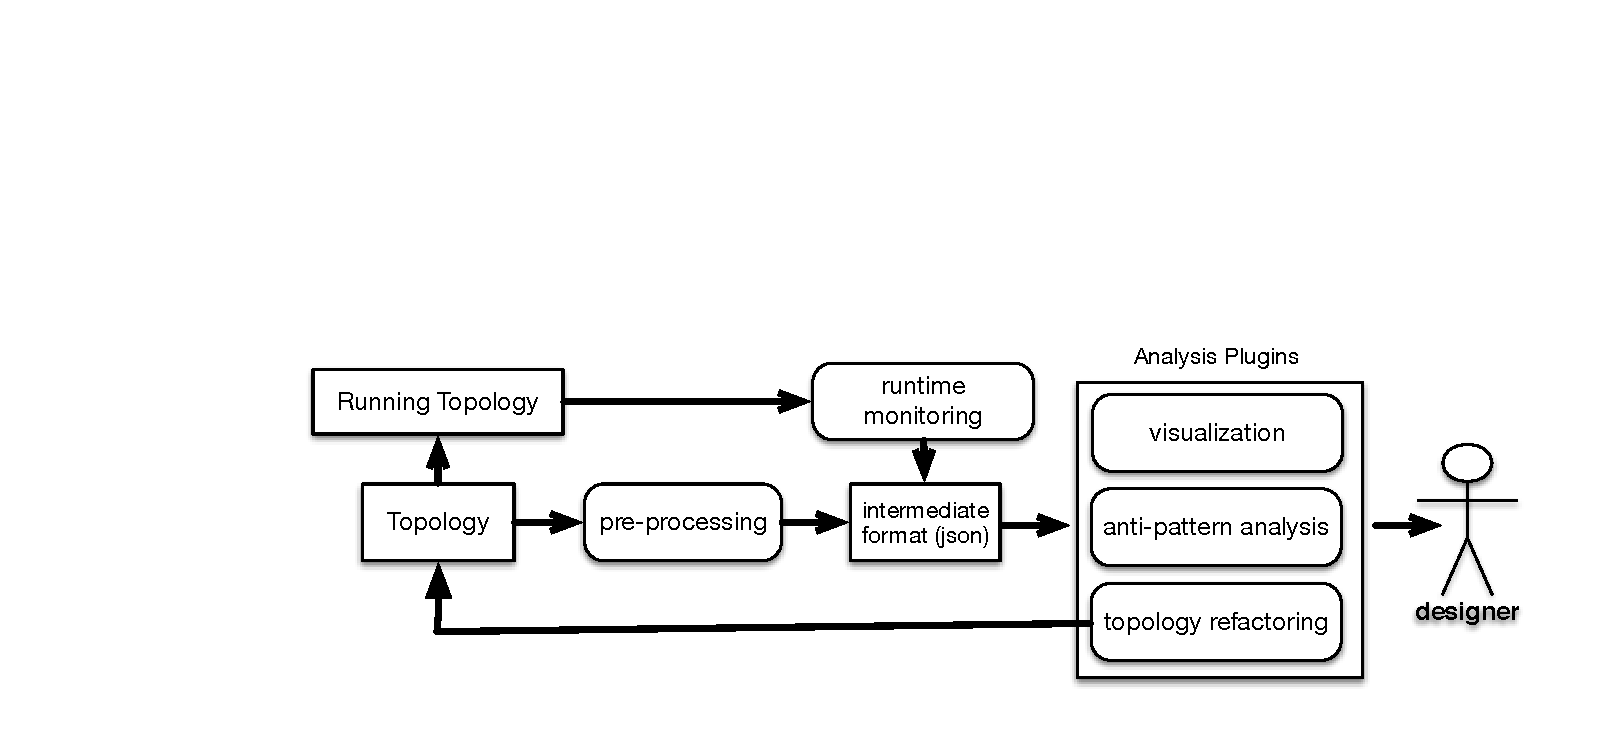
\includegraphics[width=8cm]{images/ostia-arch}
		\caption{OSTIA extensible architecture.}
		\label{fig:ostia-arch}
	\end{center}
\end{figure}